% Use the following line _only_ if you're still using LaTeX 2.09.
%\documentstyle[icml2014,epsf,natbib]{article}
% If you rely on Latex2e packages, like most modern people use this:
\documentclass{article}

% use Times
\usepackage{times}
% For figures
\usepackage{graphicx} % more modern
%\usepackage{epsfig} % less modern
\usepackage{subfigure} 

% For citations
\usepackage{natbib}

% For algorithms
%\usepackage{algorithm}
%\usepackage{algorithmic}
%\usepackage{algorithmicx}

% As of 2011, we use the hyperref package to produce hyperlinks in the
% resulting PDF.  If this breaks your system, please commend out the
% following usepackage line and replace \usepackage{icml2014} with
% \usepackage[nohyperref]{icml2014} above.
\usepackage{hyperref}

% Packages hyperref and algorithmic misbehave sometimes.  We can fix
% this with the following command.
\newcommand{\theHalgorithm}{\arabic{algorithm}}

% Employ the following version of the ``usepackage'' statement for
% submitting the draft version of the paper for review.  This will set
% the note in the first column to ``Under review.  Do not distribute.''
\usepackage{format/icml2014} 
% Employ this version of the ``usepackage'' statement after the paper has
% been accepted, when creating the final version.  This will set the
% note in the first column to ``Proceedings of the...''
%\usepackage[accepted]{icml2014}

\usepackage{times}
\usepackage{hyperref}
\usepackage{url}
\usepackage{color}
\usepackage{preamble}
\definecolor{mydarkblue}{rgb}{0,0.08,0.45}
\hypersetup{ %
    pdftitle={},
    pdfauthor={},
    pdfsubject={},
    pdfkeywords={},
    pdfborder=0 0 0,
    pdfpagemode=UseNone,
    colorlinks=true,
    linkcolor=mydarkblue,
    citecolor=mydarkblue,
    filecolor=mydarkblue,
    urlcolor=mydarkblue,
    pdfview=FitH}
    
    
\usepackage{amsmath, amsfonts, bm, lipsum, capt-of}
\usepackage{natbib, xcolor, wrapfig, booktabs, multirow, caption}
\DeclareCaptionType{copyrightbox}
\usepackage{float}


%\renewcommand{\baselinestretch}{0.99}

\def\ie{i.e.\ }
\def\eg{e.g.\ }
\let\oldemptyset\emptyset
\let\emptyset\varnothing

%\author{
%James Robert Lloyd\\
%University of Cambridge\\
%Department of Engineering\\
%\texttt{jrl44@cam.ac.uk}
%\And
%David Duvenaud\\
%University of Cambridge \\
%Department of Engineering \\
%\texttt{dkd23@cam.ac.uk}
%\And
%Roger Grosse\\
%M.I.T.\\
%Brain and Cognitive Sciences \\
%\texttt{rgrosse@mit.edu}
%\And
%Joshua B. Tenenbaum\\
%M.I.T.\\
%Brain and Cognitive Sciences \\
%\texttt{jbt@mit.edu}
%\And
%Zoubin Ghahramani\\
%University of Cambridge \\
%Department of Engineering \\
%\texttt{zoubin@eng.cam.ac.uk}
%}

\newcommand{\fix}{\marginpar{FIX}}
\newcommand{\new}{\marginpar{NEW}}

\setlength{\marginparwidth}{0.6in}
%%%%%%%%%%%%%%%%%%%%%%%%%%%%%%%%%%%%%%%%%%%%%%%%%%%%%%%%%%
%%%% EDITING HELPER FUNCTIONS  %%%%%%%%%%%%%%%%%%%%%%%%%%%
%%%%%%%%%%%%%%%%%%%%%%%%%%%%%%%%%%%%%%%%%%%%%%%%%%%%%%%%%%

%% NA: needs attention (rough writing whose correctness needs to be verified)
%% TBD: instructions for how to fix a gap ("Describe the propagation by ...")
%% PROBLEM: bug or missing crucial bit 

%% use \fXXX versions of these macros to put additional explanation into a footnote.  
%% The idea is that we don't want to interrupt the flow of the paper or make it 
%% impossible to read because there are a bunch of comments.

%% NA's (and TBDs, those less crucially) should be written so 
%% that they flow with the text.

\definecolor{WowColor}{rgb}{.75,0,.75}
\definecolor{SubtleColor}{rgb}{0,0,.50}

% inline
\newcommand{\NA}[1]{\textcolor{SubtleColor}{ {\tiny \bf ($\star$)} #1}}
\newcommand{\LATER}[1]{\textcolor{SubtleColor}{ {\tiny \bf ($\dagger$)} #1}}
\newcommand{\TBD}[1]{\textcolor{SubtleColor}{ {\tiny \bf (!)} #1}}
\newcommand{\PROBLEM}[1]{\textcolor{WowColor}{ {\bf (!!)} {\bf #1}}}

% as margin notes

\newcounter{margincounter}
\newcommand{\displaycounter}{{\arabic{margincounter}}}
\newcommand{\incdisplaycounter}{{\stepcounter{margincounter}\arabic{margincounter}}}

\newcommand{\fTBD}[1]{\textcolor{SubtleColor}{$\,^{(\incdisplaycounter)}$}\marginpar{\tiny\textcolor{SubtleColor}{ {\tiny $(\displaycounter)$} #1}}}

\newcommand{\fPROBLEM}[1]{\textcolor{WowColor}{$\,^{((\incdisplaycounter))}$}\marginpar{\tiny\textcolor{WowColor}{ {\bf $\mathbf{((\displaycounter))}$} {\bf #1}}}}

\newcommand{\fLATER}[1]{\textcolor{SubtleColor}{$\,^{(\incdisplaycounter\dagger)}$}\marginpar{\tiny\textcolor{SubtleColor}{ {\tiny $(\displaycounter\dagger)$} #1}}}


%% For submission, make all render blank.
%\renewcommand{\LATER}[1]{}
%\renewcommand{\fLATER}[1]{}
%\renewcommand{\TBD}[1]{}
%\renewcommand{\fTBD}[1]{}
%\renewcommand{\PROBLEM}[1]{}
%\renewcommand{\fPROBLEM}[1]{}
%\renewcommand{\NA}[1]{#1}  % Note, NA's pass through!


% The \icmltitle you define below is probably too long as a header.
% Therefore, a short form for the running title is supplied here:
\icmltitlerunning{Automatic construction and natural-language summarization of additive nonparametric models -- supplementary material}

\begin{document} 

\twocolumn[
\icmltitle{Automatic construction and natural-language summarization\\of additive nonparametric models -- supplementary material}

% It is OKAY to include author information, even for blind
% submissions: the style file will automatically remove it for you
% unless you've provided the [accepted] option to the icml2014
% package.
\icmlauthor{Your Name}{email@yourdomain.edu}
\icmladdress{Your Fantastic Institute,
            314159 Pi St., Palo Alto, CA 94306 USA}
\icmlauthor{Your CoAuthor's Name}{email@coauthordomain.edu}
\icmladdress{Their Fantastic Institute,
            27182 Exp St., Toronto, ON M6H 2T1 CANADA}

% You may provide any keywords that you 
% find helpful for describing your paper; these are used to populate 
% the "keywords" metadata in the PDF but will not be shown in the document
\icmlkeywords{}

\vskip 0.3in
]

\allowdisplaybreaks


\appendix


\section{Kernel equations}

Here we give exact formlae for the kernels used in the language.

For scalar-valued inputs, the zero ($\emptyset$), white noise ($\kWN$), constant ($\kC$), linear ($\kLin$), squared exponential ($\kSE$), and periodic kernels ($\kPer$) are defined as follows:
%
\begin{eqnarray}
\kernel_{\emptyset}(\inputVar, \inputVar') =& 0 \\
\kernel_{\kWN}(\inputVar, \inputVar') =& \sigma^2\delta_{\inputVar, \inputVar'} \\
\kernel_{\kC}(\inputVar, \inputVar') =& \sigma^2 \\
\kernel_{\kLin}(\inputVar, \inputVar') =& \sigma^2(\inputVar - \ell)(\inputVar' - \ell) \\
\kernel_{\kSE}(\inputVar, \inputVar') =& \sigma^2\exp\left(-\frac{(\inputVar - \inputVar')^2}{2\ell^2}\right) \\
\kernel_{\kPer}(\inputVar, \inputVar') =&  \sigma^2\frac{\exp\left(\frac{\cos\frac{2 \pi (\inputVar - \inputVar')}{p}}{\ell^2}\right) - I_0\left(\frac{1}{\ell^2}\right)}{\exp\left(\frac{1}{\ell^2}\right) - I_0\left(\frac{1}{\ell^2}\right)}
\end{eqnarray}
%
where $\delta_{\inputVar, \inputVar'}$ is the Kronecker delta and $I_0$ is the modified Bessel function of the first kind of order 0.





\section{Derivation of Component Marginal Variance}

In this section, we derive the posterior marginal variance and covariance of the additive components of a \gp{}.  These formulas let us plot the marginal variance of each component separately.  These formulas can also be used to examine the posterior covariance between pairs of components.

Let us assume that our function $\vf$ is a sum of two functions, $\vf_1$ and $\vf_2$, where $\vf = \vf_1 + \vf_2$.  If $\vf_1$ and $\vf_2$ are a priori independent, and $\vf_1 \sim \gp( \vmu_1, k_1)$ and $\vf_2 \sim \gp( \vmu_2, k_2)$, then
\begin{align}
\left[ \begin{array}{c} \vf_1 \\ \vf_1^\star \\ \vf_2 \\ \vf_2^\star \\ \vf \\ \vf^\star \end{array} \right]
\sim
\Nt{
\left[ \begin{array}{c} \vmu_1 \\ \vmu_1^\star \\ \vmu_2 \\ \vmu_2^\star \\ \vmu_1 + \vmu_2 \\ \vmu_1^\star + \vmu_2^\star \end{array} \right]
}
{K
}
\end{align}

where
\begin{align}
 K = \left[ \begin{array}{cccccc} 
\vk_1 & \vk_1^\star & 0 & 0 & \vk_1 & \vk_1^\star \\ 
\vk_1^\star & \vk_1^{\star\star} & 0 & 0 & \vk_1^\star & \vk_1^{\star\star} \\
0 & 0 & \vk_2 & \vk_2^\star & \vk_2 & \vk_2^\star \\ 
0 & 0 & \vk_2^\star & \vk_2^{\star\star} & \vk_2^\star & \vk_2^{\star\star} \\
\vk_1 & \vk_1^\star & \vk_2 & \vk_2^\star & \vk_1 + \vk_2 & \vk_1^\star + \vk_2^\star \\ 
\vk_1^\star & \vk_1^{\star\star}  & \vk_2^\star & \vk_2^{\star\star}  & \vk_1^\star + \vk_2^\star & \vk_1^{\star\star} + \vk_2^{\star\star}\\
\end{array} \right]
\end{align}

and 

\begin{align}
\vk_1 & = k_1( \vX, \vX ) \\
\vk_1^\star & = k_1( \vX^\star, \vX ) \\
\vk_1^{\star\star} & = k_1( \vX^\star, \vX^\star )
\end{align} 

By the formula for Gaussian conditionals:
\begin{align}
\vx_A | \vx B \sim \mathcal{N} \big( & \vmu_A + \vSigma_{AB} \vSigma_{BB}\inv \left( \vx_B - \vmu_B \right), \\
& \vSigma_{AA} - \vSigma_{AB} \vSigma_{BB}\inv \vSigma_{BA} \big),
\end{align}
we get that the conditional variance of a Gaussian conditioned on its sum with another Gaussian is given by
\begin{align}
\vf_1^\star | \vf \sim \mathcal{N} \big( &\vmu_1^\star + \vk_1^{\star\tra} (\vK_1 + \vK_2)\inv \left( \vf - \vmu_1 - \vmu_2 \right), \\
 & \vk_1^{\star\star} - \vk_1^{\star\tra} (\vK_1 + \vK_2)\inv \vk_1^\star \big).
\end{align}

The covariance between the two components, conditioned on their sum is given by:
\begin{align}
\cov(\vf_1^\star, \vf_2^\star) | \vf = - \vk_1^{\star\tra} (\vK_1 + \vK_2)\inv \vk_2^\star
\end{align}

These formulae express the posterior model uncertainty about different components of the signal, integrating over the possible configurations of the other components.









\section{Search}

\subsection{Overview}

The ABCDE search algorithm starts with the kernel equal to the noise kernel, $\kWN$.
New kernel expressions are generated by applying search operators to the current kernel.
When new base kernels are proposed by the search operators, their parameters are randomly initialised with several restarts.
Parameters are then optimized by conjugate gradients to maximise the likelihood of the data conditioned on the kernel parameters.
The kernels are then scored by the Bayesian information criterion and the top scoring kernel is selected as the new kernel.
The search then proceeds by applying the search operators to the new kernel.

Unless stated otherwise, 10 random restarts were used for parameter initialisation and searches were run to a depth of 10.

\subsection{Operators}

The original GPSS algorithm included the following search operators
%
\begin{eqnarray}
\mathcal{S} &\to& \mathcal{S} + \mathcal{B} \\
\mathcal{S} &\to& \mathcal{S} \times \mathcal{B} \\
\mathcal{B} &\to& \mathcal{B'}
\end{eqnarray}
%
where $\mathcal{S}$ represents any kernel subexpression and $\mathcal{B}$ is any base kernel within a kernel expression \ie the search operators represent addition, multiplication and replacement.

To accommodate changepoint/window operators we introduce the following additional operators
%
\begin{eqnarray}
\mathcal{S} &\to& \kCP(\mathcal{S},\mathcal{S}) \\
\mathcal{S} &\to& \kCW(\mathcal{S},\mathcal{S}) \\
\mathcal{S} &\to& \kCW(\mathcal{S},\kC) \\
\mathcal{S} &\to& \kCW(\kC,\mathcal{S})
\end{eqnarray}
%
where $\kC$ is the constant kernel.
The last two operators result in a kernel only applying outside or within a certain region.

Based on experience with typical paths followed by the search algorithm of GPSS we introduced the following operators
%
\begin{eqnarray}
\mathcal{S} &\to& \mathcal{S} \times (\mathcal{B} + \kC)\\
\mathcal{S} &\to& \mathcal{B}\\
\mathcal{S} + \mathcal{S'} &\to& \mathcal{S}\\
\mathcal{S} \times \mathcal{S'} &\to& \mathcal{S}
\end{eqnarray}
%
where $\mathcal{S'}$ represents any other kernel expression.
Their introduction is currently not rigorously justified.
Further research into the search strategy would be a profitable area of future study.

\section{Translation of kernel functions}

\section{Numerical evaluation}

\subsection{Tabels of standardised RMSEs}

Ordered by dataset.

\begin{table}
\begin{tabular}{|c|c|c|c|c|c|}
\hline
GPSS & TCI & SP & SE & CP & EL \\
\hline
1.00 & 1.26 & 2.00 & 3.07 & 3.12 & 5.09\\
1.00 & 1.50 & 1.09 & 1.50 & 1.75 & 3.22\\
1.00 & 1.00 & 1.08 & 2.68 & 2.68 & 26.15\\
1.09 & 1.00 & 1.00 & 1.00 & 1.37 & 1.59\\
1.00 & 1.06 & 1.08 & 1.01 & 1.01 & 1.49\\
1.10 & 1.00 & 1.61 & 1.53 & 1.63 & 5.77\\
1.55 & 1.00 & 1.02 & 1.00 & 1.52 & 2.40\\
1.00 & 1.24 & 1.26 & 1.49 & 1.49 & 2.43\\
1.00 & 1.06 & 1.08 & 1.30 & 1.29 & 2.84\\
1.00 & 1.10 & 1.06 & 1.14 & 1.27 & 39.27\\
1.08 & 1.00 & 1.36 & 2.33 & 2.82 & 3.14\\
1.00 & 1.20 & 1.76 & 1.79 & 1.79 & 1.93\\
1.00 & 1.03 & 1.03 & 1.03 & 1.02 & 2.24\\
\hline
\end{tabular}
\caption{Interpolation standardised RMSEs}
\end{table}

\begin{table}
\begin{tabular}{|c|c|c|c|c|c|}
\hline
GPSS & TCI & SP & SE & CP & EL \\
\hline
1.14 & 1.44 & 1.00 & 4.73 & 4.80 & 3.24\\
1.00 & 1.03 & 1.21 & 1.00 & 1.03 & 2.64\\
1.09 & 1.00 & 1.03 & 1.35 & 1.35 & 1.97\\
1.07 & 3.00 & 3.00 & 3.00 & 1.00 & 1.31\\
1.00 & 1.00 & 1.03 & 1.35 & 1.35 & 1.28\\
1.00 & 2.14 & 3.38 & 4.09 & 4.17 & 6.26\\
1.66 & 1.00 & 6.14 & 1.00 & 1.97 & 274.32\\
3.10 & 2.31 & 1.00 & 3.13 & 3.13 & 1.41\\
1.00 & 1.52 & 1.61 & 2.90 & 3.14 & 2.73\\
1.00 & 1.80 & 1.43 & 1.61 & 2.25 & 1.97\\
1.30 & 1.35 & 2.15 & 1.03 & 1.00 & 1.34\\
1.00 & 1.47 & 1.46 & 1.75 & 1.74 & 1.82\\
3.03 & 3.12 & 3.63 & 3.16 & 5.83 & 1.00\\
\hline
\end{tabular}
\caption{Extrapolation standardised RMSEs}
\end{table}

\subsection{Tabels of standardised RMSEs - 2 variant version}

\begin{table}
\begin{tabular}{|c|c|c|c|c|c|c|}
\hline
GPSS & GPSS.int & TCI & SP & SE & CP & EL \\
\hline
1.04 & 1.00 & 1.32 & 2.09 & 3.20 & 3.25 & 5.30\\
1.00 & 1.27 & 1.50 & 1.09 & 1.50 & 1.75 & 3.22\\
1.00 & 1.00 & 1.00 & 1.09 & 2.69 & 2.69 & 26.20\\
1.09 & 1.04 & 1.00 & 1.00 & 1.00 & 1.37 & 1.59\\
1.00 & 1.06 & 1.06 & 1.08 & 1.01 & 1.01 & 1.49\\
1.50 & 1.00 & 1.37 & 2.19 & 2.09 & 2.23 & 7.88\\
1.55 & 1.50 & 1.00 & 1.02 & 1.00 & 1.52 & 2.40\\
1.00 & 1.30 & 1.24 & 1.26 & 1.49 & 1.49 & 2.43\\
1.00 & 1.09 & 1.06 & 1.08 & 1.30 & 1.29 & 2.84\\
1.08 & 1.00 & 1.19 & 1.15 & 1.23 & 1.38 & 42.56\\
1.13 & 1.00 & 1.05 & 1.42 & 2.44 & 2.96 & 3.29\\
1.00 & 1.15 & 1.20 & 1.76 & 1.79 & 1.79 & 1.93\\
1.00 & 1.10 & 1.03 & 1.03 & 1.03 & 1.02 & 2.24\\
\hline
\end{tabular}
\caption{Interpolation standardised RMSEs}
\end{table}

\begin{table}
\begin{tabular}{|c|c|c|c|c|c|c|}
\hline
GPSS & GPSS.int & TCI & SP & SE & CP & EL \\
\hline
1.14 & 2.10 & 1.44 & 1.00 & 4.73 & 4.80 & 3.24\\
1.00 & 1.26 & 1.03 & 1.21 & 1.00 & 1.03 & 2.64\\
1.40 & 1.00 & 1.29 & 1.32 & 1.74 & 1.74 & 2.54\\
1.07 & 1.18 & 3.00 & 3.00 & 3.00 & 1.00 & 1.31\\
1.00 & 1.00 & 1.00 & 1.03 & 1.35 & 1.35 & 1.28\\
1.00 & 2.03 & 2.14 & 3.38 & 4.09 & 4.17 & 6.26\\
2.98 & 1.00 & 1.80 & 11.04 & 1.80 & 3.54 & 493.30\\
3.10 & 1.88 & 2.31 & 1.00 & 3.13 & 3.13 & 1.41\\
1.00 & 2.05 & 1.52 & 1.61 & 2.90 & 3.14 & 2.73\\
1.00 & 1.45 & 1.80 & 1.43 & 1.61 & 2.25 & 1.97\\
1.30 & 1.22 & 1.35 & 2.15 & 1.03 & 1.00 & 1.34\\
1.06 & 1.00 & 1.56 & 1.54 & 1.85 & 1.84 & 1.93\\
3.03 & 4.00 & 3.12 & 3.63 & 3.16 & 5.83 & 1.00\\
\hline
\end{tabular}
\caption{Extrapolation standardised RMSEs}
\end{table}





\subsubsection{Heteroscedasticity}

In the original GPSS the heteroscedasticity of the airline dataset was partially captured by the $\kLin \times \kSE \times \kRQ$ term which was modeling short term variation.
This term was also modeling the medium term variations in the data (an example of $\kRQ$ capturing multiple lengthscales) forcing a compromise of parameter values\fTBD{This may also be a result of not distributing products during the search - not entirely sure} resulting in the variance of the residuals decreasing (see figure~\ref{fig:not_hetero} from old GPSS) rather than increasing with the data (see new figure~\ref{fig:hetero}).\fTBD{The noise variance is too high due to a mathematical error in the original version}

\begin{figure}[h]
\centering
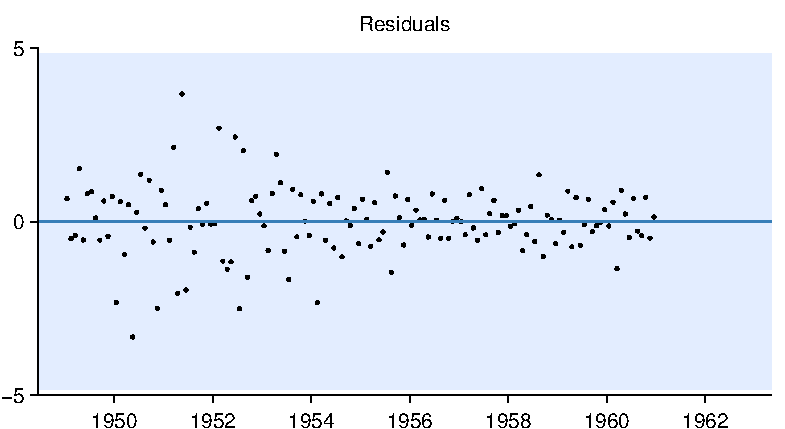
\includegraphics[width=0.98\columnwidth]{figures/old-gpss/01-airline-months_resid}
\caption{Old GPSS - heteroscedasticity not captured and variance larger than residuals.}
\label{fig:not_hetero}
\end{figure}

\begin{figure}[h]
\centering
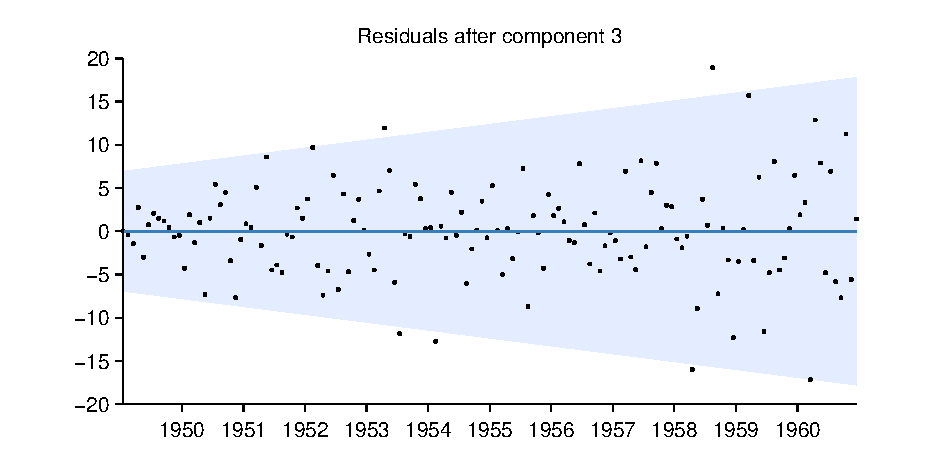
\includegraphics[width=0.98\columnwidth]{figures/01-airline/01-airline_3_anti_cum}
\caption{New GPSS - heteroscedasticity captured and mostly appropriate.}
\label{fig:hetero}
\end{figure}

Introducing $\kWN$ as a base kernel allows heteroscedasticity to be explicitly modelled\fTBD{we now have a delta likelihood function rather than always assuming homoscedastic Gaussian noise} rather than having to approximate it with components that can represent short lengthscales.




\subsubsection{Removal of $\kRQ$}

GPML describes the $\kRQ$ as ``a scale mixture of \kSE covariance functions with different characteristic length-scales''.
To exactly specify this scale mixture would require an equation or plot.
One could summarise this information with descriptions like `90\% of the length-scales are between $x$ and $y$' but I do not think there is any common language that would express what is happening exactly.

Also the $\kRQ$ kernel can model smooth trends and very short term variation in one component.
What was previously one component (figure \ref{fig:RQ}) is now two (figures \ref{fig:medium} and \ref{fig:short}) in new GPSS.
This feels more interpretable to me, but this is subjective and maybe subtle.

\begin{figure}[h]
\centering
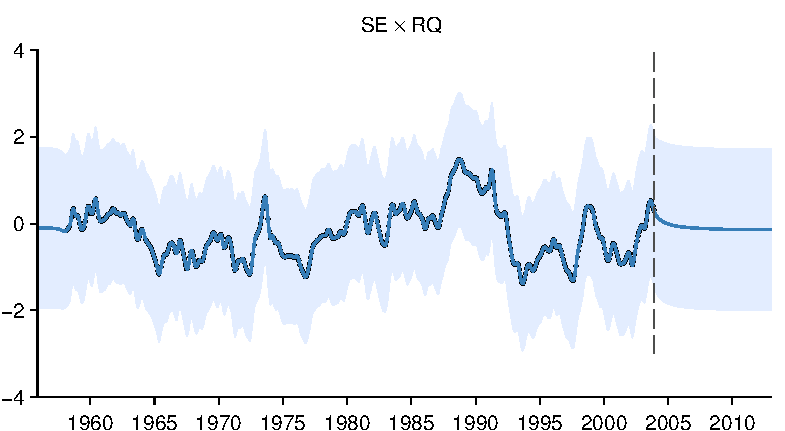
\includegraphics[width=0.98\columnwidth]{figures/old-gpss/03-mauna2003-s_3}
\caption{Old GPSS - many lengthscales in one component.}
\label{fig:RQ}
\end{figure}

\begin{figure}[h]
\centering
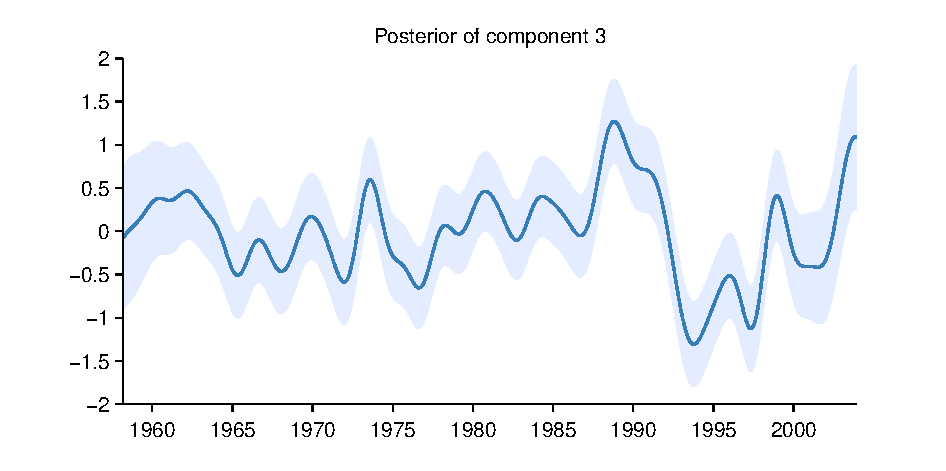
\includegraphics[width=0.98\columnwidth]{figures/03-mauna/03-mauna_3}
\caption{New GPSS - medium term variation.}
\label{fig:medium}
\end{figure}

\begin{figure}[h]
\centering
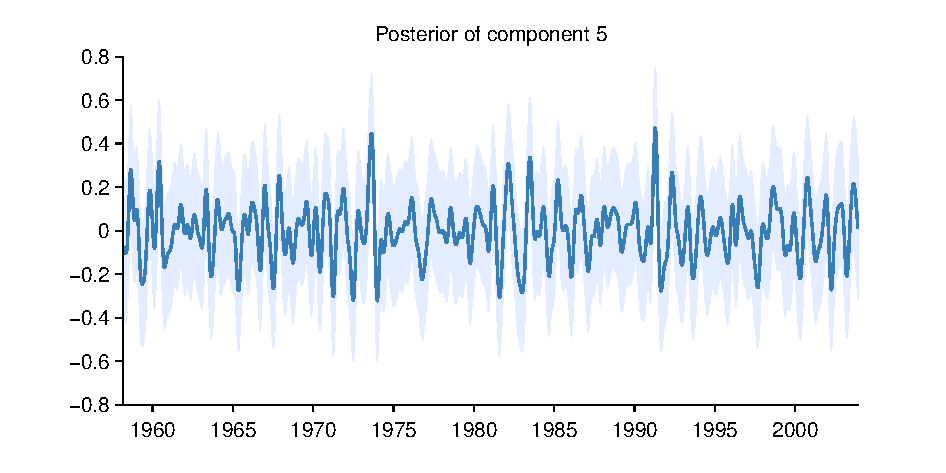
\includegraphics[width=0.98\columnwidth]{figures/03-mauna/03-mauna_5}
\caption{New GPSS - very short term variation.}
\label{fig:short}
\end{figure}

More convincing hopefully is the plot in figure~\ref{fig:RQ_bad} which shows a fit to data representing sales of mink fur.
The kernel is $\kRQ \times \kPer$\fTBD{redundant multiplicative constant kernels were not removed in the version of the algorithm that produced this figure}.
The extrapolation shows that it has captured the near exact periodicity (\ie a long lengthscale phenomenon) but the interpolation shows it has also captured short term variation (it has joined the dots!).
Combining these scales of variation does not seem interpretable\fTBD{I tried for quite some time to avoid this fit to the data before convincing myself that $\kRQ$ was the problem rather than anything else}.

\begin{figure}[h]
\centering
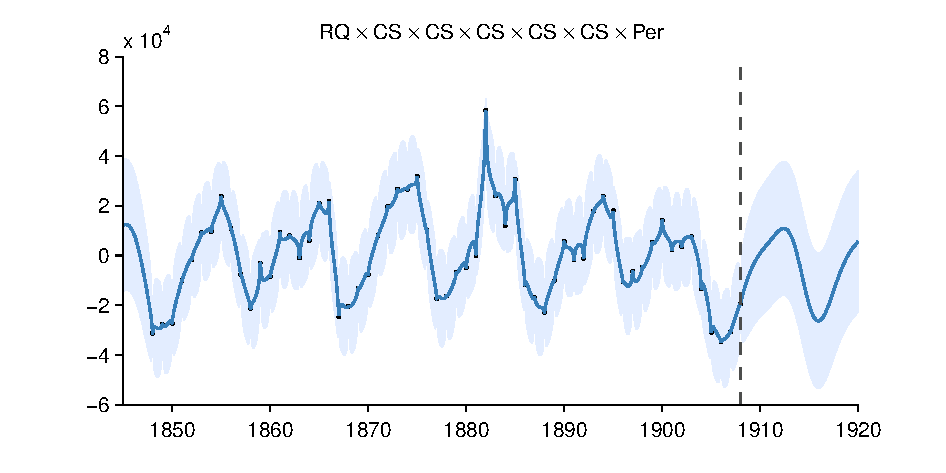
\includegraphics[width=0.98\columnwidth]{figures/old-gpss/fur-sales-mink-h-b-co-18481911_1}
\caption{Old GPSS - the trend and noise in one component.}
\label{fig:RQ_bad}
\end{figure}

\subsection{An improved periodic kernel}

We introduce a new periodic kernel defined by
\begin{equation}
\kernel_\kPer(x, x') = \kernel_\kPer(\tau) =  \sigma^2\frac{\exp\left(\frac{\cos\frac{2 \pi \tau}{p}}{\ell^2}\right) - I_0\left(\frac{1}{\ell^2}\right)}{\exp\left(\frac{1}{\ell^2}\right) - I_0\left(\frac{1}{\ell^2}\right)}
\label{eq:periodic}
\end{equation}
where $\tau := x - x'$ and $I_0$ is the modified Bessel function of the first kind of order 0.
It is linearly related to the original periodic kernel \TBD{cite something?} but has the following elegant properties.

\paragraph{Cosine limit}

A simple application of l'H\^opital's rule shows that
\begin{equation}
\kernel_\kPer(\tau) \to \sigma^2\cos\left(\frac{2 \pi \tau}{p}\right) \quad \textrm{as} \quad\ell \to \infty.
\end{equation}
It was recently demonstrated \citep{WilAda13} that any stationary kernel can be arbitrarily well approximated by kernels with syntax\fTBD{RG: Syntax $\to$ expression, structure, family?}
\begin{equation}
\sum \kSE \times \cos
\end{equation}
by appealing to Bochner's theorem \citep{bochner1959lectures}.
By using this new periodic kernel our language of kernels also attains this completeness property.

\paragraph{No power at zero frequency}

The kernel defined by equation~\eqref{eq:periodic} has a Fourier transform of zero when evaluated at zero.
Therefore, functions drawn from a \gp{} with this kernel will have zero mean.
In contrast, the previous periodic kernel defined a prior over a zero mean periodic function plus an independent constant function.
For the purposes of description we find it more interpretable to separate zero mean periodicity and constant functions.
\NA{
cite Sheffield's orthogonal RKHS work?
}



\section{Extra Experimental Results}
\paragraph{Interpolation}

To test the ability of the methods to interpolate, we randomly divided each data set into equal amounts of training data and testing data.
We trained each algorithm on the training half of the data, produced predictions for the remaining half and then computed the root mean squared error (RMSE).
The values of the RMSEs are then standardised by dividing by the smallest RMSE for each data set \ie the best performance on each data set will have a value of 1.

Figure~\ref{fig:box_interp} shows the standardised RMSEs for the different algorithms.
The box plots show that all quartiles of the distribution of standardised RMSEs are lower for GPSS.
\NA{ The median for GPSS is 1, and it was the best performing algorithm on 9 of the datasets.
However, the largest outliers of GPSS, TCI and SP are all quite similar in value.}

\begin{figure*}[h]
\centering
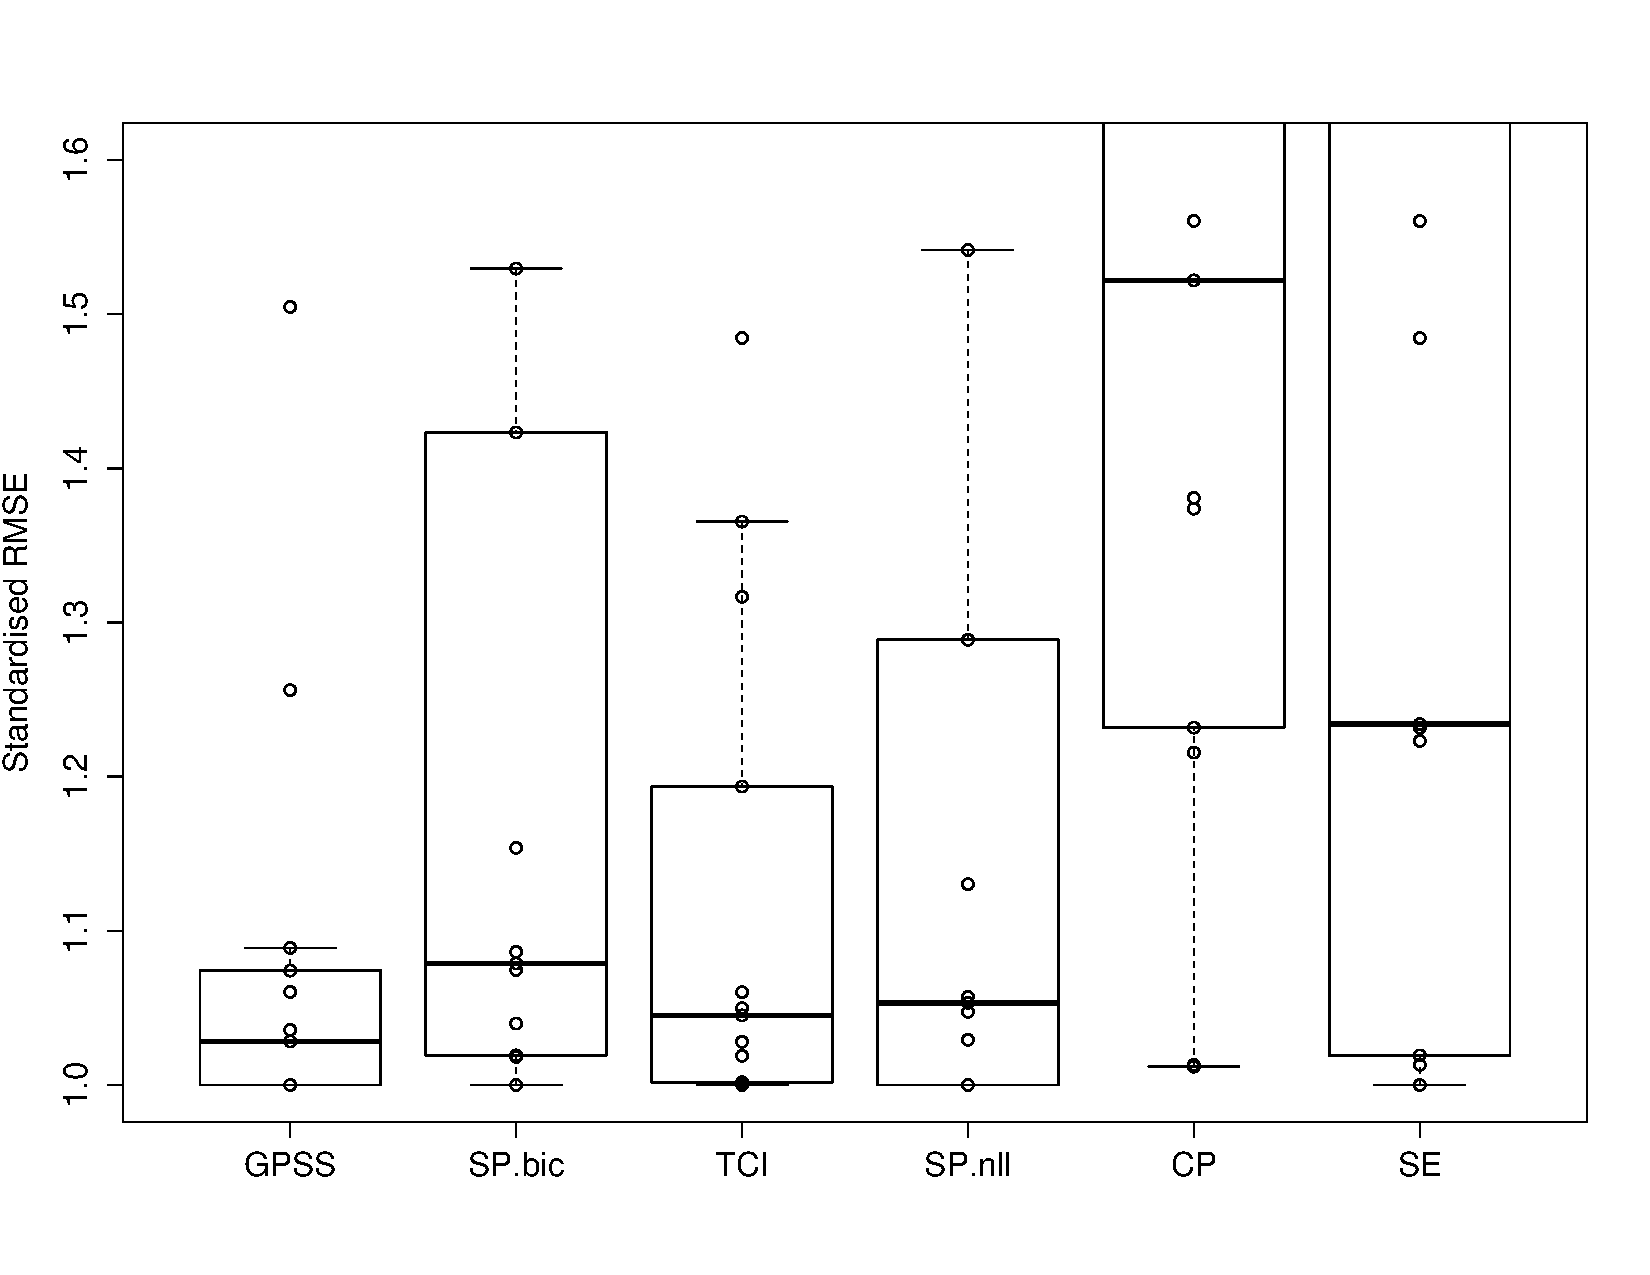
\includegraphics[width=\textwidth]{figures/box_interp}
\caption{
Box plot of standardised RMSE (best performance = 1) on 13 interpolation tasks.
}
\label{fig:box_interp}
\end{figure*}

CP performs slightly worse than SE despite being strictly more general than SE.
The introduction of changepoints allows for more structured models, but it introduces parametric forms into the regression models (\ie the sigmoids expressing the changepoints).
This results in worse interpolations at the locations of the change points, suggesting that a more robust modelling language would require a more flexible class of changepoint shapes or improved inference (\eg fully Bayesian inference over the location and shape of the changepoint\TBD{Cite something - anyone know any good references?}).

EL is not suited to this task and performs poorly.
The models learned by EL tend to capture only broad trends of the data since the fine details are not well explained by parametric forms.

\begin{figure}[h]
\centering
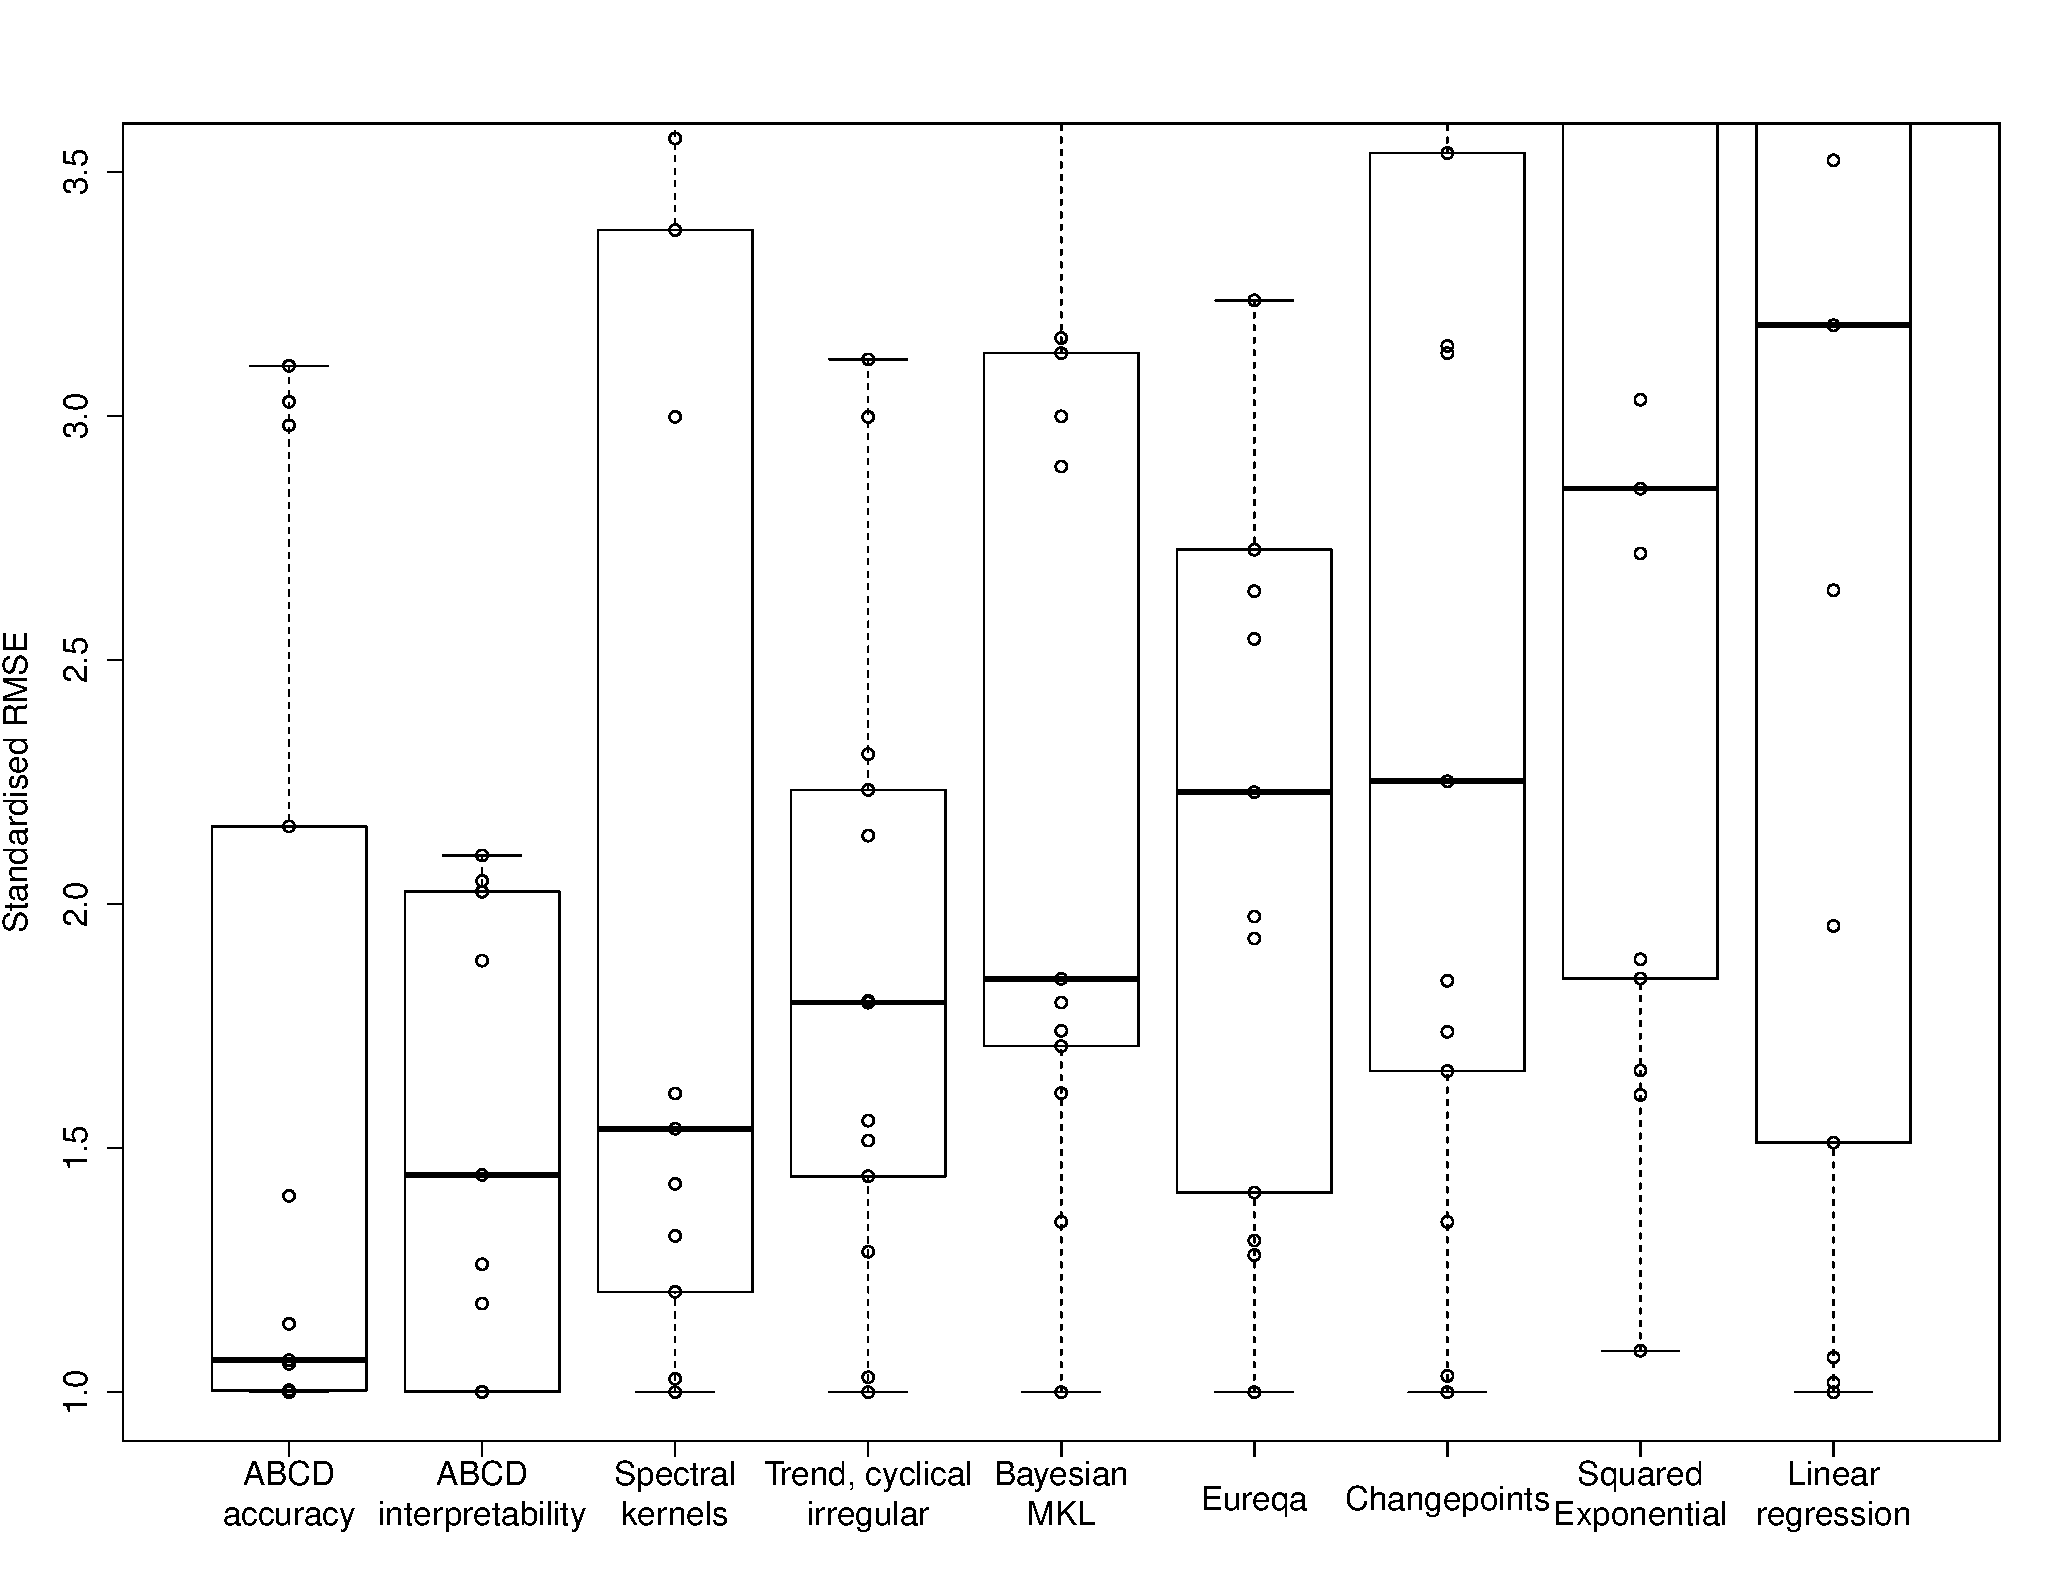
\includegraphics[width=\columnwidth]{figures/box_extrap}
\caption{
Raw data, and box plot of standardised extrapolation RMSE (best performance = 1).
Ordered by median.
}
\label{fig:box_extrap}
\end{figure}



\begin{figure}[h]
\centering
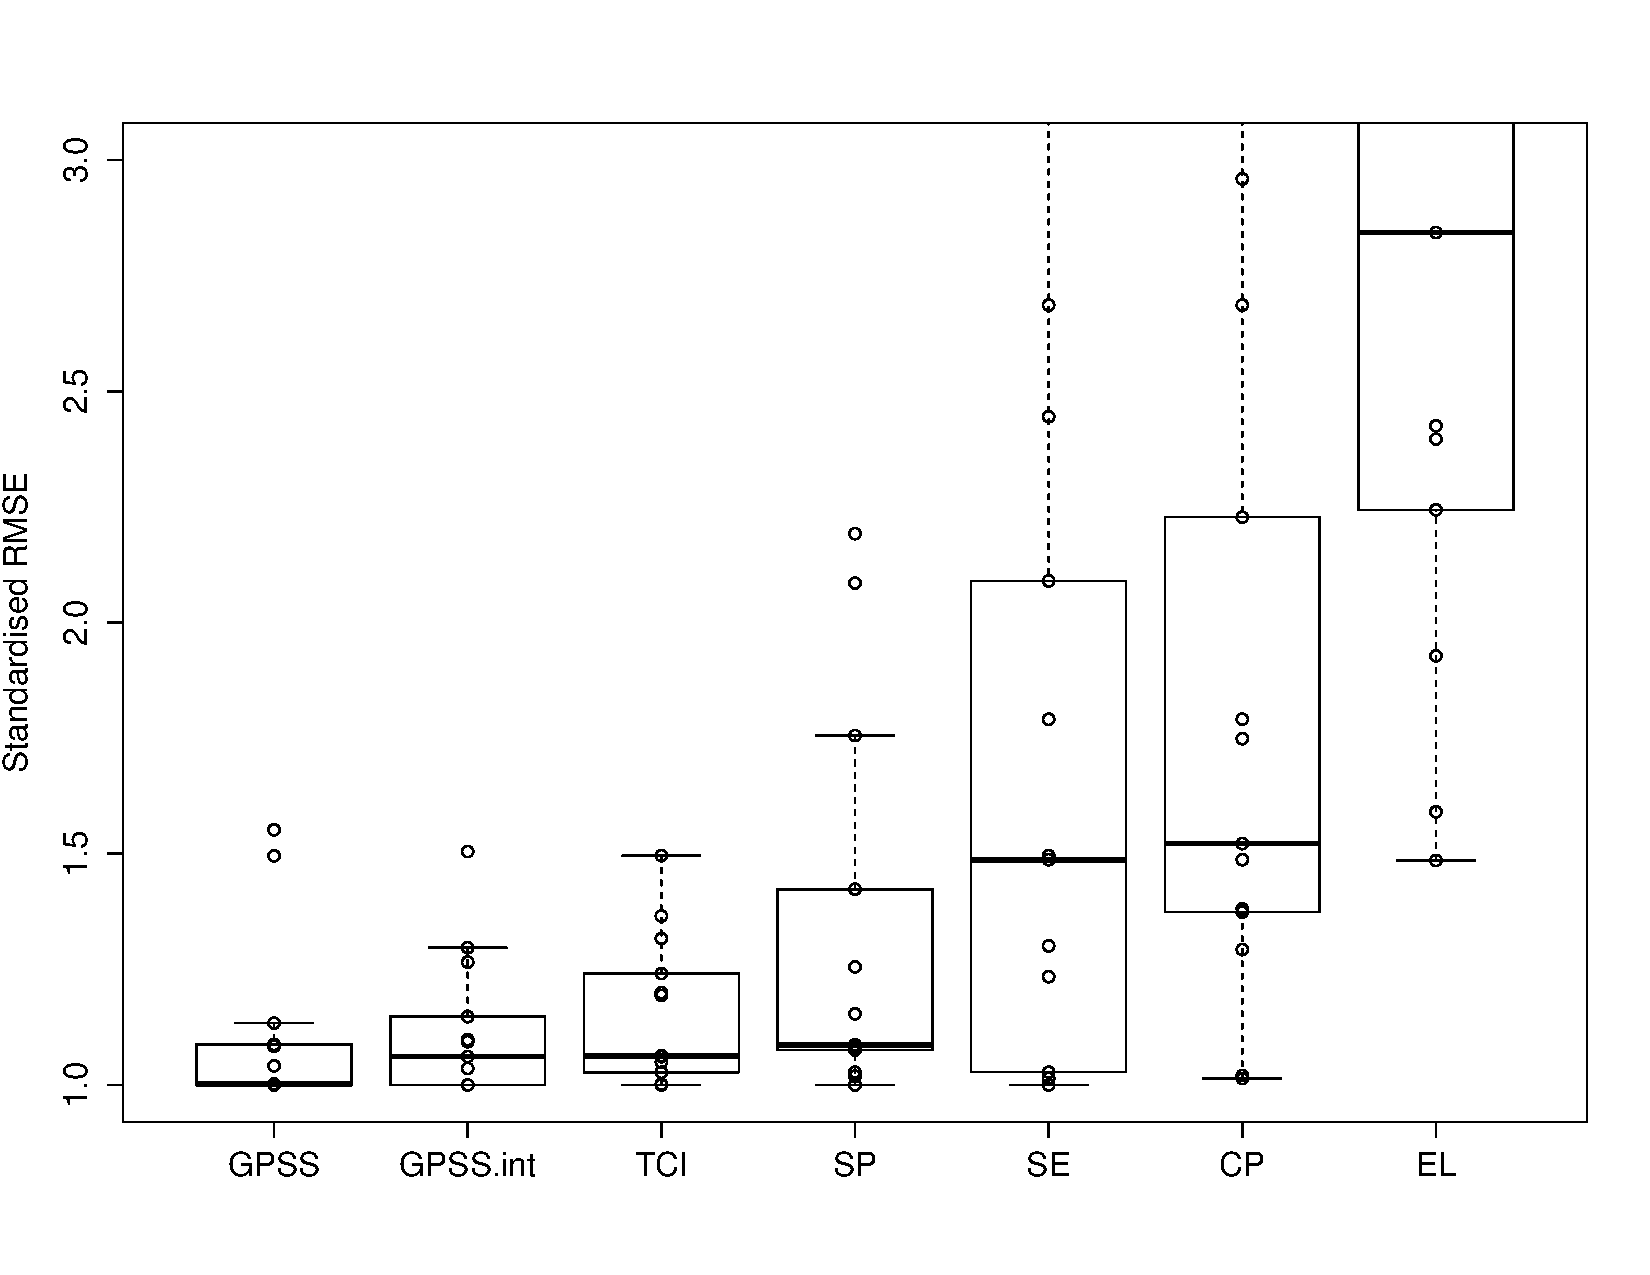
\includegraphics[width=\columnwidth]{figures/box_interp_dist}
\caption{
Raw data, and box plot of standardised interpolation RMSE (best performance = 1).
}
\label{fig:box_interp_dist}
\end{figure}






\section{Improvements to Language}

\subsubsection{Changepoints and changewindows}

Old GPSS could not capture changepoints evidenced by these solar irradiance data residuals in figure~\ref{fig:not_cp}.
New GPSS can do changepoints (see later section).

\begin{figure}[h]
\centering
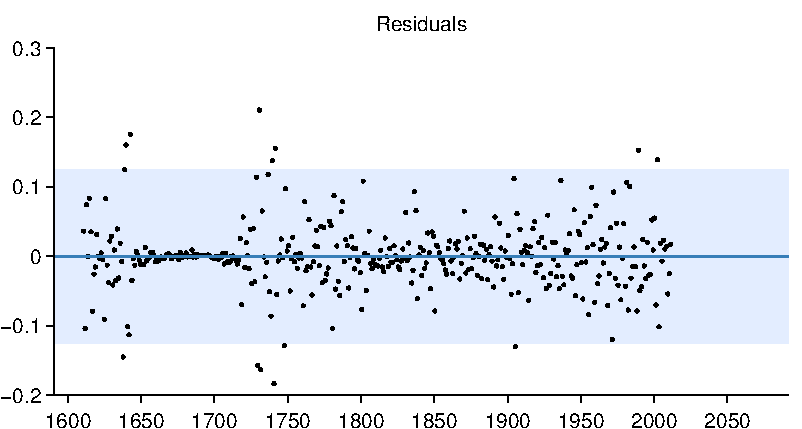
\includegraphics[width=0.98\columnwidth]{figures/old-gpss/02-solar-s_resid}
\caption{Old GPSS - these residuals need a changepoint.}
\label{fig:not_cp}
\end{figure}

\subsubsection{Removing constants}

The first two components in the old GPSS decomposition of airline were
\begin{itemize}
  \item $\kSE \times \kLin_1'$
  \item $\kSE \times \kLin_2' \times \kPer'$
\end{itemize}
where primes represent old defintions of the kernels.
The linear kernels have different parameters (indicated by subscripts) but the $\kSE$ is the same in both products.

Using the new versions of the kernels (removing constants) these expressions become
\begin{itemize}
  \item $\kSE \times \kLin_1 + \kSE$
  \item $\kSE \times \kLin_2 \times \kPer + \kSE \times \kLin_2 +  \kSE \times \kPer + \kSE$
\end{itemize}
which is undesirable in two ways.
Firstly, both of these expressions contain the same $\kSE$ as an additive component resulting in anti-correlation in the posterior; contrast figures \ref{fig:anti_corr_1} and \ref{fig:anti_corr_2} with figures \ref{fig:monotonic} and \ref{fig:lin_periodic}.

Secondly, the second component is a sum of four terms and is therefore rather a mouthful to describe.
It is the sum of an approximately periodic function with approximately linearly increasing amplitude, a smooth function with linearly increasing marginal standard deviation, an approximately periodic function and a smooth function!

The removal of constants results in base kernels which are atomic from the point of view of description \fTBD{In the way they are currently translated at least} and they make anti-correlation less likely\fTBD{however, they are not orthogonal in any sense so anti-correlation can still happen - I'm not sure how to avoid this or whether it is inevitable}.

\begin{figure}[h]
\centering
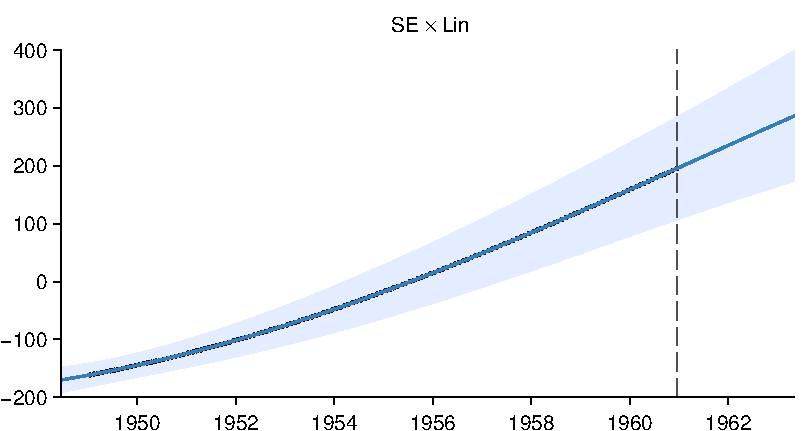
\includegraphics[width=0.98\columnwidth]{figures/old-gpss/01-airline-months_1}
\caption{Old GPSS - uncertainty is in fact anti-correlation.}
\label{fig:anti_corr_1}
\end{figure}

\begin{figure}[h]
\centering
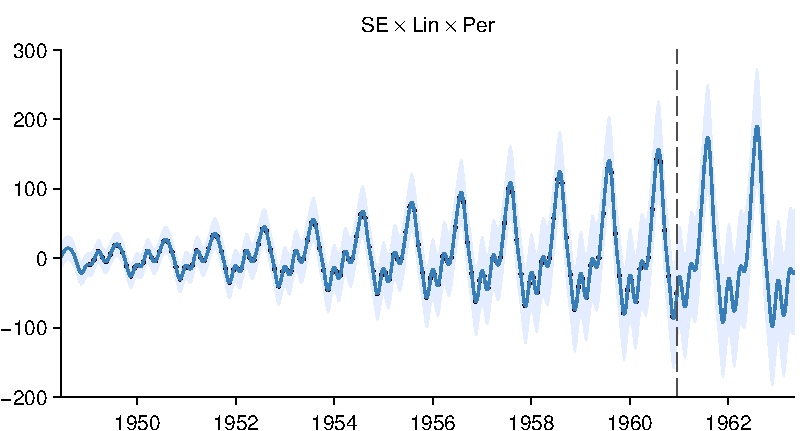
\includegraphics[width=0.98\columnwidth]{figures/old-gpss/01-airline-months_2}
\caption{Old GPSS - uncertainty is in fact anti-correlation.}
\label{fig:anti_corr_2}
\end{figure}

\paragraph{Removal of $\kRQ$}
The $\kRQ$ kernel is equivalent to a mixture of $\kSE$ covariance functions with different length-scales.
In preliminary testing we observed that this allowed the kernel to simultaneously model aspects of the data that might be considered signal and noise.
We therefore removed this kernel to improve the interpretability of the models produced.


\end{document} 



Let us assume that our function $\vf$ is a sum of two functions, $\vf_1$ and $\vf_2$, where $\vf = \vf_1 + \vf_2$.  If $\vf_1$ and $\vf_2$ are a priori independent, and $\vf_1 \sim \gp( \vmu_1, k_1)$ and $\vf_2 \sim \gp( \vmu_2, k_2)$, then
\begin{align}
\left[ \begin{array}{c} \vf_1 \\ \vf_1^\star \\ \vf_2 \\ \vf_2^\star \\ \vf \\ \vf^\star \end{array} \right]
\sim
\Nt{
\left[ \begin{array}{c} \vmu_1 \\ \vmu_1^\star \\ \vmu_2 \\ \vmu_2^\star \\ \vmu_1 + \vmu_2 \\ \vmu_1^\star + \vmu_2^\star \end{array} \right]
}
{\left[ \begin{array}{cccccc} 
\vk_1 & \vk_1^\star & 0 & 0 & \vk_1 & \vk_1^\star \\ 
\vk_1^\star & \vk_1^{\star\star} & 0 & 0 & \vk_1^\star & \vk_1^{\star\star} \\
0 & 0 & \vk_2 & \vk_2^\star & \vk_2 & \vk_2^\star \\ 
0 & 0 & \vk_2^\star & \vk_2^{\star\star} & \vk_2^\star & \vk_2^{\star\star} \\
\vk_1 & \vk_1^\star & \vk_2 & \vk_2^\star & \vk_1 + \vk_2 & \vk_1^\star + \vk_2^\star \\ 
\vk_1^\star & \vk_1^{\star\star}  & \vk_2^\star & \vk_2^{\star\star}  & \vk_1^\star + \vk_2^\star & \vk_1^{\star\star} + \vk_2^{\star\star}\\
\end{array} \right]
}
\end{align}
where $\vk_1 = k_1( \vX, \vX )$ and $\vk_1^\star = k_1( \vX^\star, \vX )$. 

By the formula for Gaussian conditionals:
\begin{align}
\vx_A | \vx B \sim \Nt{\vmu_A + \vSigma_{AB} \vSigma_{BB}\inv \left( \vx_B - \vmu_B \right) }
{\vSigma_{AA} - \vSigma_{AB} \vSigma_{BB}\inv \vSigma_{BA} },
\end{align}
we get that the conditional variance of a Gaussian conditioned on its sum with another Gaussian is given by
\begin{align}
\vf_1^\star | \vf \sim \Nt{\vmu_1^\star + \vk_1^{\star\tra} (\vK_1 + \vK_2)\inv \left( \vf - \vmu_1 - \vmu_2 \right) }
{\vk_1^{\star\star} - \vk_1^{\star\tra} (\vK_1 + \vK_2)\inv \vk_1^\star }.
\end{align}

The covariance between the two components, conditioned on their sum is given by:
\begin{align}
\cov(\vf_1^\star, \vf_2^\star) | \vf = - \vk_1^{\star\tra} (\vK_1 + \vK_2)\inv \vk_2^\star
\end{align}

These formulae express the posterior model uncertainty about different components of the signal, integrating over the possible configurations of the other components.


